\documentclass[10pt]{article}
\usepackage[paperwidth=14.8in,paperheight=6.3in,margin=0.18in]{geometry}
\usepackage{amsmath,amssymb,bm}
\usepackage{tikz}
\usetikzlibrary{arrows.meta,positioning,calc,fit,backgrounds}
\pagestyle{empty}

\definecolor{inputgray}{RGB}{76,84,92}
\definecolor{predblue}{RGB}{42,104,145}
\definecolor{predgreen}{RGB}{42,124,91}
\definecolor{controlred}{RGB}{181,74,58}
\definecolor{controlorange}{RGB}{196,116,42}
\definecolor{fitpurple}{RGB}{102,75,145}

\begin{document}
\centering
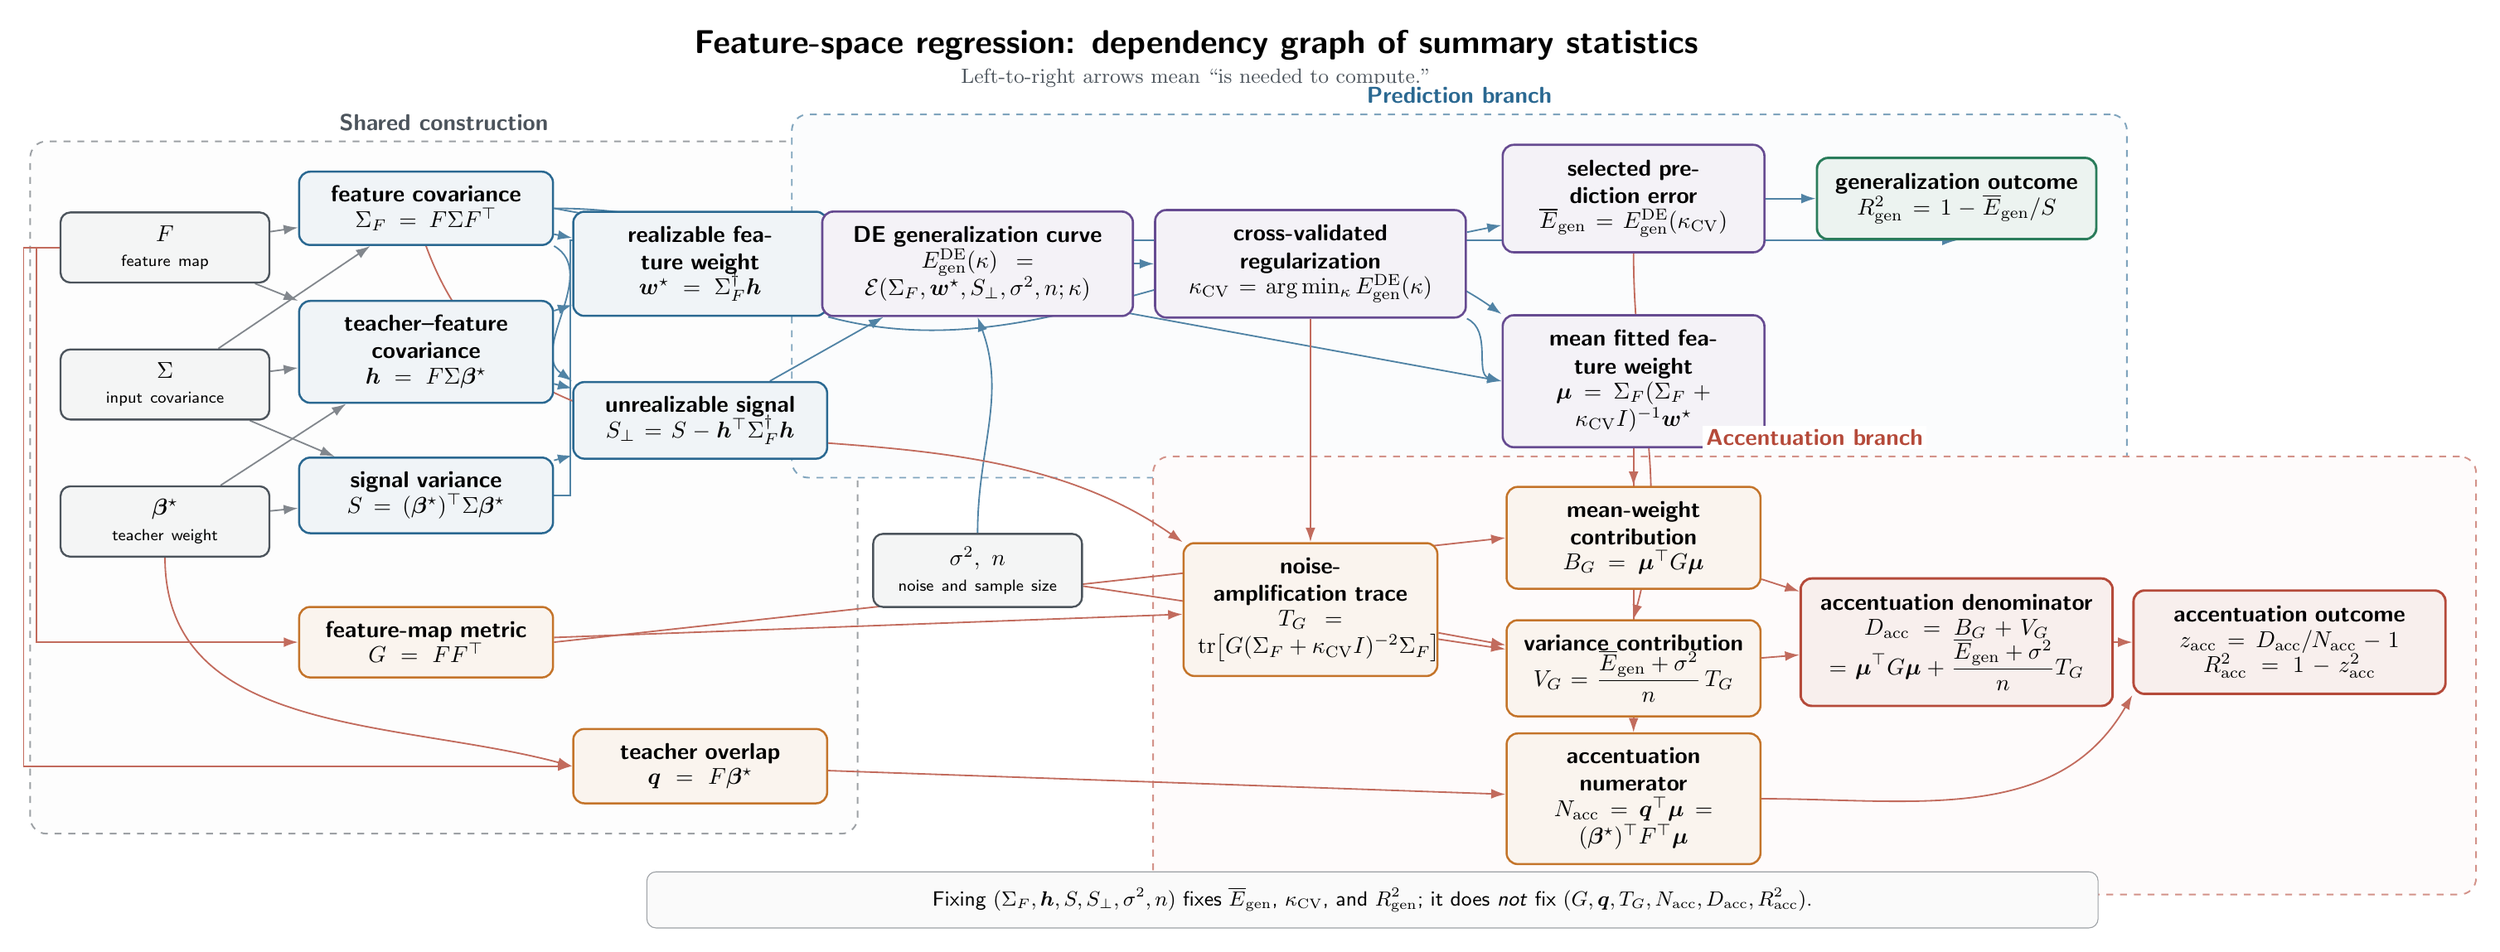
\begin{tikzpicture}[
  x=1cm,y=1cm,
  font=\sffamily,
  >=Latex,
  dep/.style={-{Latex[length=2.2mm,width=1.5mm]},
              draw=inputgray!70,line width=0.66pt},
  preddep/.style={dep,draw=predblue!82},
  accdep/.style={dep,draw=controlred!82},
  input/.style={draw=inputgray,line width=0.85pt,rounded corners=1.5mm,
                fill=inputgray!6,text width=2.8cm,minimum height=0.92cm,
                align=center,inner sep=2mm},
  pstat/.style={draw=predblue,line width=0.9pt,rounded corners=1.7mm,
                fill=predblue!7,text width=3.45cm,minimum height=1.08cm,
                align=center,inner sep=2.2mm},
  astat/.style={draw=controlorange,line width=0.9pt,rounded corners=1.7mm,
                fill=controlorange!8,text width=3.45cm,minimum height=1.08cm,
                align=center,inner sep=2.2mm},
  modelstat/.style={draw=fitpurple,line width=0.95pt,rounded corners=1.7mm,
                    fill=fitpurple!7,text width=4.3cm,minimum height=1.08cm,
                    align=center,inner sep=2.3mm},
  compactfit/.style={modelstat,text width=3.55cm},
  predout/.style={draw=predgreen,line width=1.05pt,rounded corners=1.7mm,
                  fill=predgreen!9,text width=3.8cm,minimum height=1.12cm,
                  align=center,inner sep=2.4mm},
  accout/.style={draw=controlred,line width=1.05pt,rounded corners=1.7mm,
                 fill=controlred!9,text width=4.3cm,minimum height=1.12cm,
                 align=center,inner sep=2.4mm},
  group/.style={draw,line width=0.7pt,dashed,rounded corners=2.5mm,
                inner sep=4.5mm}
]

% Title.
\node[font=\sffamily\Large\bfseries] at (4.8,6.90)
  {Feature-space regression: dependency graph of summary statistics};
\node[font=\small,text=inputgray] at (4.8,6.40)
  {Left-to-right arrows mean ``is needed to compute.''};

% --------------------------------------------------------------------------
% Shared construction: primitive objects and their first summaries.
% --------------------------------------------------------------------------
\node[input] (F)     at (-11.0,3.8) {$F$\\[-1pt]\scriptsize feature map};
\node[input] (Sigma) at (-11.0,1.7) {$\Sigma$\\[-1pt]\scriptsize input covariance};
\node[input] (beta)  at (-11.0,-0.4) {$\bm\beta^\star$\\[-1pt]\scriptsize teacher weight};

\node[pstat] (C) at (-7.0,4.4) {
  \textbf{feature covariance}\\[-1pt]
  $\Sigma_F=F\Sigma F^\top$
};
\node[pstat] (h) at (-7.0,2.2) {
  \textbf{teacher--feature covariance}\\[-1pt]
  $\bm h=F\Sigma\bm\beta^\star$
};
\node[pstat] (S) at (-7.0,0.0) {
  \textbf{signal variance}\\[-1pt]
  $S=(\bm\beta^\star)^\top\Sigma\bm\beta^\star$
};

\node[pstat] (wstar) at (-2.8,3.55) {
  \textbf{realizable feature weight}\\[-1pt]
  $\bm w^\star=\Sigma_F^\dagger\bm h$
};
\node[pstat] (Sperp) at (-2.8,1.15) {
  \textbf{unrealizable signal}\\[-1pt]
  $S_\perp=S-\bm h^\top \Sigma_F^\dagger\bm h$
};

% Control-specific summaries are kept at the bottom of the shared-input region.
\node[astat] (G) at (-7.0,-2.25) {
  \textbf{feature-map metric}\\[-1pt]
  $G=FF^\top$
};
\node[astat] (q) at (-2.8,-4.15) {
  \textbf{teacher overlap}\\[-1pt]
  $\bm q=F\bm\beta^\star$
};

% Noise/sample size live at the split between the two downstream branches.
\node[input] (noise) at (1.45,-1.15) {
  $\sigma^2,\ n$\\[-1pt]\scriptsize noise and sample size
};

% --------------------------------------------------------------------------
% Prediction branch (upper lane).
% --------------------------------------------------------------------------
\node[modelstat] (Ecurve) at (1.45,3.55) {
  \textbf{DE generalization curve}\\[-1pt]
  $E_{\rm gen}^{\rm DE}(\kappa)
   =\mathcal E(\Sigma_F,\bm w^\star,S_\perp,\sigma^2,n;\kappa)$
};
\node[modelstat] (kcv) at (6.55,3.55) {
  \textbf{cross-validated regularization}\\[-1pt]
  $\kappa_{\rm CV}=\arg\min_\kappa E_{\rm gen}^{\rm DE}(\kappa)$
};
\node[compactfit] (Ecv) at (11.5,4.55) {
  \textbf{selected prediction error}\\[-1pt]
  $\overline E_{\rm gen}=E_{\rm gen}^{\rm DE}(\kappa_{\rm CV})$
};
\node[compactfit] (mu) at (11.5,1.75) {
  \textbf{mean fitted feature weight}\\[-1pt]
  $\bm\mu=\Sigma_F(\Sigma_F+\kappa_{\rm CV}I)^{-1}\bm w^\star$
};
\node[predout] (Rgen) at (16.45,4.55) {
  \textbf{generalization outcome}\\[-1pt]
  $R_{\rm gen}^2=1-\overline E_{\rm gen}/S$
};

% --------------------------------------------------------------------------
% Accentuation branch (lower lane).  The denominator is explicitly factored
% into mean-weight and variance contributions to keep arrows local.
% --------------------------------------------------------------------------
\node[astat] (TG) at (6.55,-1.75) {
  \textbf{noise-amplification trace}\\[-1pt]
  $T_G=\operatorname{tr}\!\left[G(\Sigma_F+\kappa_{\rm CV}I)^{-2}\Sigma_F\right]$
};
\node[astat] (BG) at (11.5,-0.65) {
  \textbf{mean-weight contribution}\\[-1pt]
  $B_G=\bm\mu^\top G\bm\mu$
};
\node[astat] (VG) at (11.5,-2.65) {
  \textbf{variance contribution}\\[-1pt]
  $V_G=\dfrac{\overline E_{\rm gen}+\sigma^2}{n}\,T_G$
};
\node[astat] (Nacc) at (11.5,-4.65) {
  \textbf{accentuation numerator}\\[-1pt]
  $N_{\rm acc}=\bm q^\top\bm\mu
   =(\bm\beta^\star)^\top F^\top\bm\mu$
};
\node[accout] (Dacc) at (16.45,-2.25) {
  \textbf{accentuation denominator}\\[-1pt]
  $D_{\rm acc}=B_G+V_G$\\[-1pt]
  $\displaystyle
   =\bm\mu^\top G\bm\mu+
   \frac{\overline E_{\rm gen}+\sigma^2}{n}T_G$
};
\node[accout] (Racc) at (21.55,-2.25) {
  \textbf{accentuation outcome}\\[-1pt]
  $z_{\rm acc}=D_{\rm acc}/N_{\rm acc}-1$\\[-1pt]
  $R_{\rm acc}^2=1-z_{\rm acc}^2$
};

% --------------------------------------------------------------------------
% Cluster backgrounds and dependency arrows.  Arrows sit behind opaque nodes.
% --------------------------------------------------------------------------
\begin{scope}[on background layer]
  \node[group,draw=inputgray!55,fill=inputgray!1,
        fit=(F)(Sigma)(beta)(C)(h)(S)(wstar)(Sperp)(G)(q)]
        (sharedgroup) {};
  \node[group,draw=predblue!60,fill=predblue!2,
        fit=(Ecurve)(kcv)(Ecv)(mu)(Rgen)] (predgroup) {};
  \node[group,draw=controlred!60,fill=controlred!2,
        fit=(TG)(BG)(VG)(Nacc)(Dacc)(Racc)] (accgroup) {};

  % Primitive inputs -> shared statistics.
  \draw[dep] (F) -- (C);
  \draw[dep] (Sigma) -- (C);
  \draw[dep] (F) -- (h);
  \draw[dep] (Sigma) -- (h);
  \draw[dep] (beta) -- (h);
  \draw[dep] (Sigma) -- (S);
  \draw[dep] (beta) -- (S);
  \draw[accdep] (F.west) -- ++(-0.35,0) |- (G.west);
  \draw[accdep] (F.west) -- ++(-0.55,0) |- (q.west);
  \draw[accdep] (beta.south) to[out=-90,in=165] (q.west);

  % Shared prediction summaries.
  \draw[preddep] (C) -- (wstar);
  \draw[preddep] (h) -- (wstar);
  \draw[preddep] (C.south east) to[out=-30,in=145] (Sperp.north west);
  \draw[preddep] (h) -- (Sperp);
  \draw[preddep] (S) -- (Sperp);

  % Upper prediction lane.
  \draw[preddep] (C.east) to[out=0,in=165] (Ecurve.west);
  \draw[preddep] (wstar) -- (Ecurve);
  \draw[preddep] (Sperp) -- (Ecurve);
  \draw[preddep] (noise.north) to[out=90,in=-70] (Ecurve.south);
  \draw[preddep] (Ecurve) -- (kcv);
  \draw[preddep] (kcv) -- (Ecv);
  \draw[preddep] (kcv.south east) to[out=-25,in=165] (mu.west);
  \draw[preddep] (C.east) -- (mu.west);
  \draw[preddep] (wstar.south east) to[out=-15,in=145] (mu.north west);
  \draw[preddep] (Ecv) -- (Rgen);
  \draw[preddep] (S.east) -- ++(0.25,0) |- (Rgen.south);

  % Lower accentuation lane.
  \draw[accdep] (G) -- (TG);
  \draw[accdep] (C.south) to[out=-70,in=145] (TG.north west);
  \draw[accdep] (kcv.south) -- (TG.north);
  \draw[accdep] (G.east) -- (BG.west);
  \draw[accdep] (mu) -- (BG);
  \draw[accdep] (TG) -- (VG);
  \draw[accdep] (Ecv.south) to[out=-90,in=75] (VG.north);
  \draw[accdep] (noise) -- (VG);
  \draw[accdep] (q) -- (Nacc);
  \draw[accdep] (mu.south) to[out=-90,in=90] (Nacc.north);
  \draw[accdep] (BG) -- (Dacc);
  \draw[accdep] (VG) -- (Dacc);
  \draw[accdep] (Dacc) -- (Racc);
  \draw[accdep] (Nacc.east) to[out=0,in=-120] (Racc.south west);
\end{scope}

% Cluster labels are placed last so no line crosses their text.
\node[font=\bfseries\sffamily,text=inputgray,
      fill=white,inner sep=1.5pt,above=1mm of sharedgroup.north]
  {Shared construction};
\node[font=\bfseries\sffamily,text=predblue,
      fill=white,inner sep=1.5pt,above=1mm of predgroup.north]
  {Prediction branch};
\node[font=\bfseries\sffamily,text=controlred,
      fill=white,inner sep=1.5pt,above=1mm of accgroup.north]
  {Accentuation branch};

% Bottom-line thesis.
\node[draw=inputgray!55,fill=black!2,rounded corners=1.4mm,
      text width=22.0cm,align=center,inner ysep=2.4mm,font=\small\sffamily]
  at (7.5,-6.20) {
  Fixing $(\Sigma_F,\bm h,S,S_\perp,\sigma^2,n)$ fixes
  $\overline E_{\rm gen}$, $\kappa_{\rm CV}$, and $R_{\rm gen}^2$;
  it does \emph{not} fix $(G,\bm q,T_G,N_{\rm acc},D_{\rm acc},R_{\rm acc}^2)$.
};

\end{tikzpicture}
\end{document}
